\subsection{LST}
Ladder Side-Tuning (LST) \cite{sung2022lst} is a recent advancement in the area of memory-efficient PEFT that has a significantly smaller memory footprint compared to other methods. The method achieves memory efficiency by circumventing the need to backpropagate through the large pre-trained backbone. Unlike other techniques that incorporate parameters into the pre-trained backbone network, LST involves training a small, separate ladder side network. This side network takes intermediate activations from the backbone network via lateral side connections (Shown in \Cref{lst-original}).

While LST represents a significant advancement in terms of memory efficiency during training, its observed performance is lower compared to other state-of-the-art (SOTA) PEFT techniques. The design of LST, which prevents the method from directly affecting the backbone's forward pass, appears to limit its ability to fully leverage the pre-training of the original model.

\begin{figure}[h]
    \centering
    %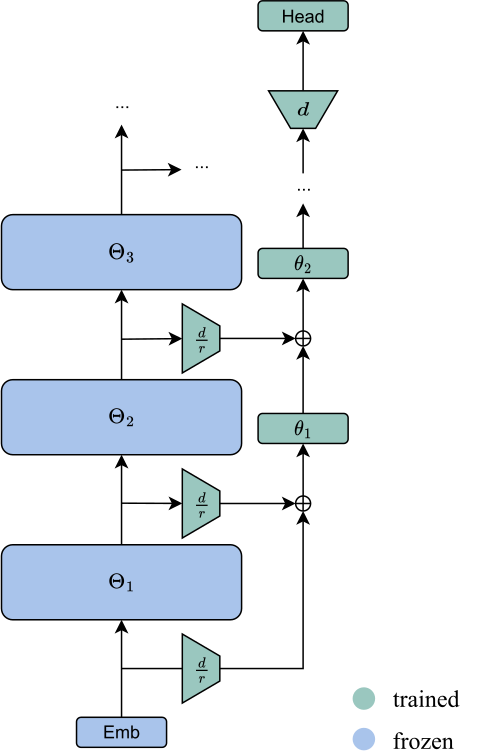
\includegraphics[width=0.7\linewidth]{assets/images/LST.png}
    \includesvg[width=0.65\linewidth]{assets/images/LST.svg}
    \caption{The original LST architecture for an encoder-only backbone. The intermediate backbone representations are downsampled to a dimension of \(d/r\), after which they are fused with the side network features. The gradients of the trainable parameters (shown in green) are computed without going through the backbone network (shown in blue).}
    \label{lst-original}
\end{figure}